%% This is an example first chapter.  You should put chapter/appendix that you
%% write into a separate file, and add a line \include{yourfilename} to
%% main.tex, where `yourfilename.tex' is the name of the chapter/appendix file.
%% You can process specific files by typing their names in at the 
%% \files=
%% prompt when you run the file main.tex through LaTeX.
\chapter{Introduction}

\section{The Glashow-Weinberg-Salam theory of Weak interactions}

\section{The SM Higgs mechanism}

\section{Extended Higgs Sector and MSSM}

\section{The W,Z, and Higgs boson production at the LHC}

\section{Monte Carlo Simulations and Cross Sections}
    
\section{The Large Hadron Collider}
The Large Hadron Collider (LHC)\cite{1748-0221-3-08-S08001} is a circular proton-proton collider located at the European Organization for Nuclear Research (CERN). The tunnel has a circumference of $26.7$ km and previously hosted the Large Electron-Positron (LEP)\cite{lep1,lep2} collider. Located at the border of France and Switzerland, the tunnel lies between $45$ m and $170$ m below the surface. The LHC is designed to collide beams of protons at centre-of-mass energy $\sqrt{s}$ of up to $14~\TeV$. While the LHC is primarily a proton-proton collider, lead (Pb) ion beams of energy of $2.3~\TeV$ per nucleon are used to produce lead-lead  and proton-lead collisions.  
 
Figure~\ref{fig:cern} shows a schematic representation of the accelerator complex at CERN. Ionized hydrogen atoms are accelerated to an energy of $50~\MeV$ in the Linac $2$ linear accelerator. Thereafter they are injected into the Proton Synchrotron Booster (PSB) and Super Proton Synchrotron (SPS) raising the energy to $25~\GeV$ and $450~\GeV$ respectively. From the SPS the protons are injected into two separate rings in discrete bunches. At the design bunch spacing of $25$ ns there are $2808$ proton bunches per beam. 

\begin{figure}[h]
\centering
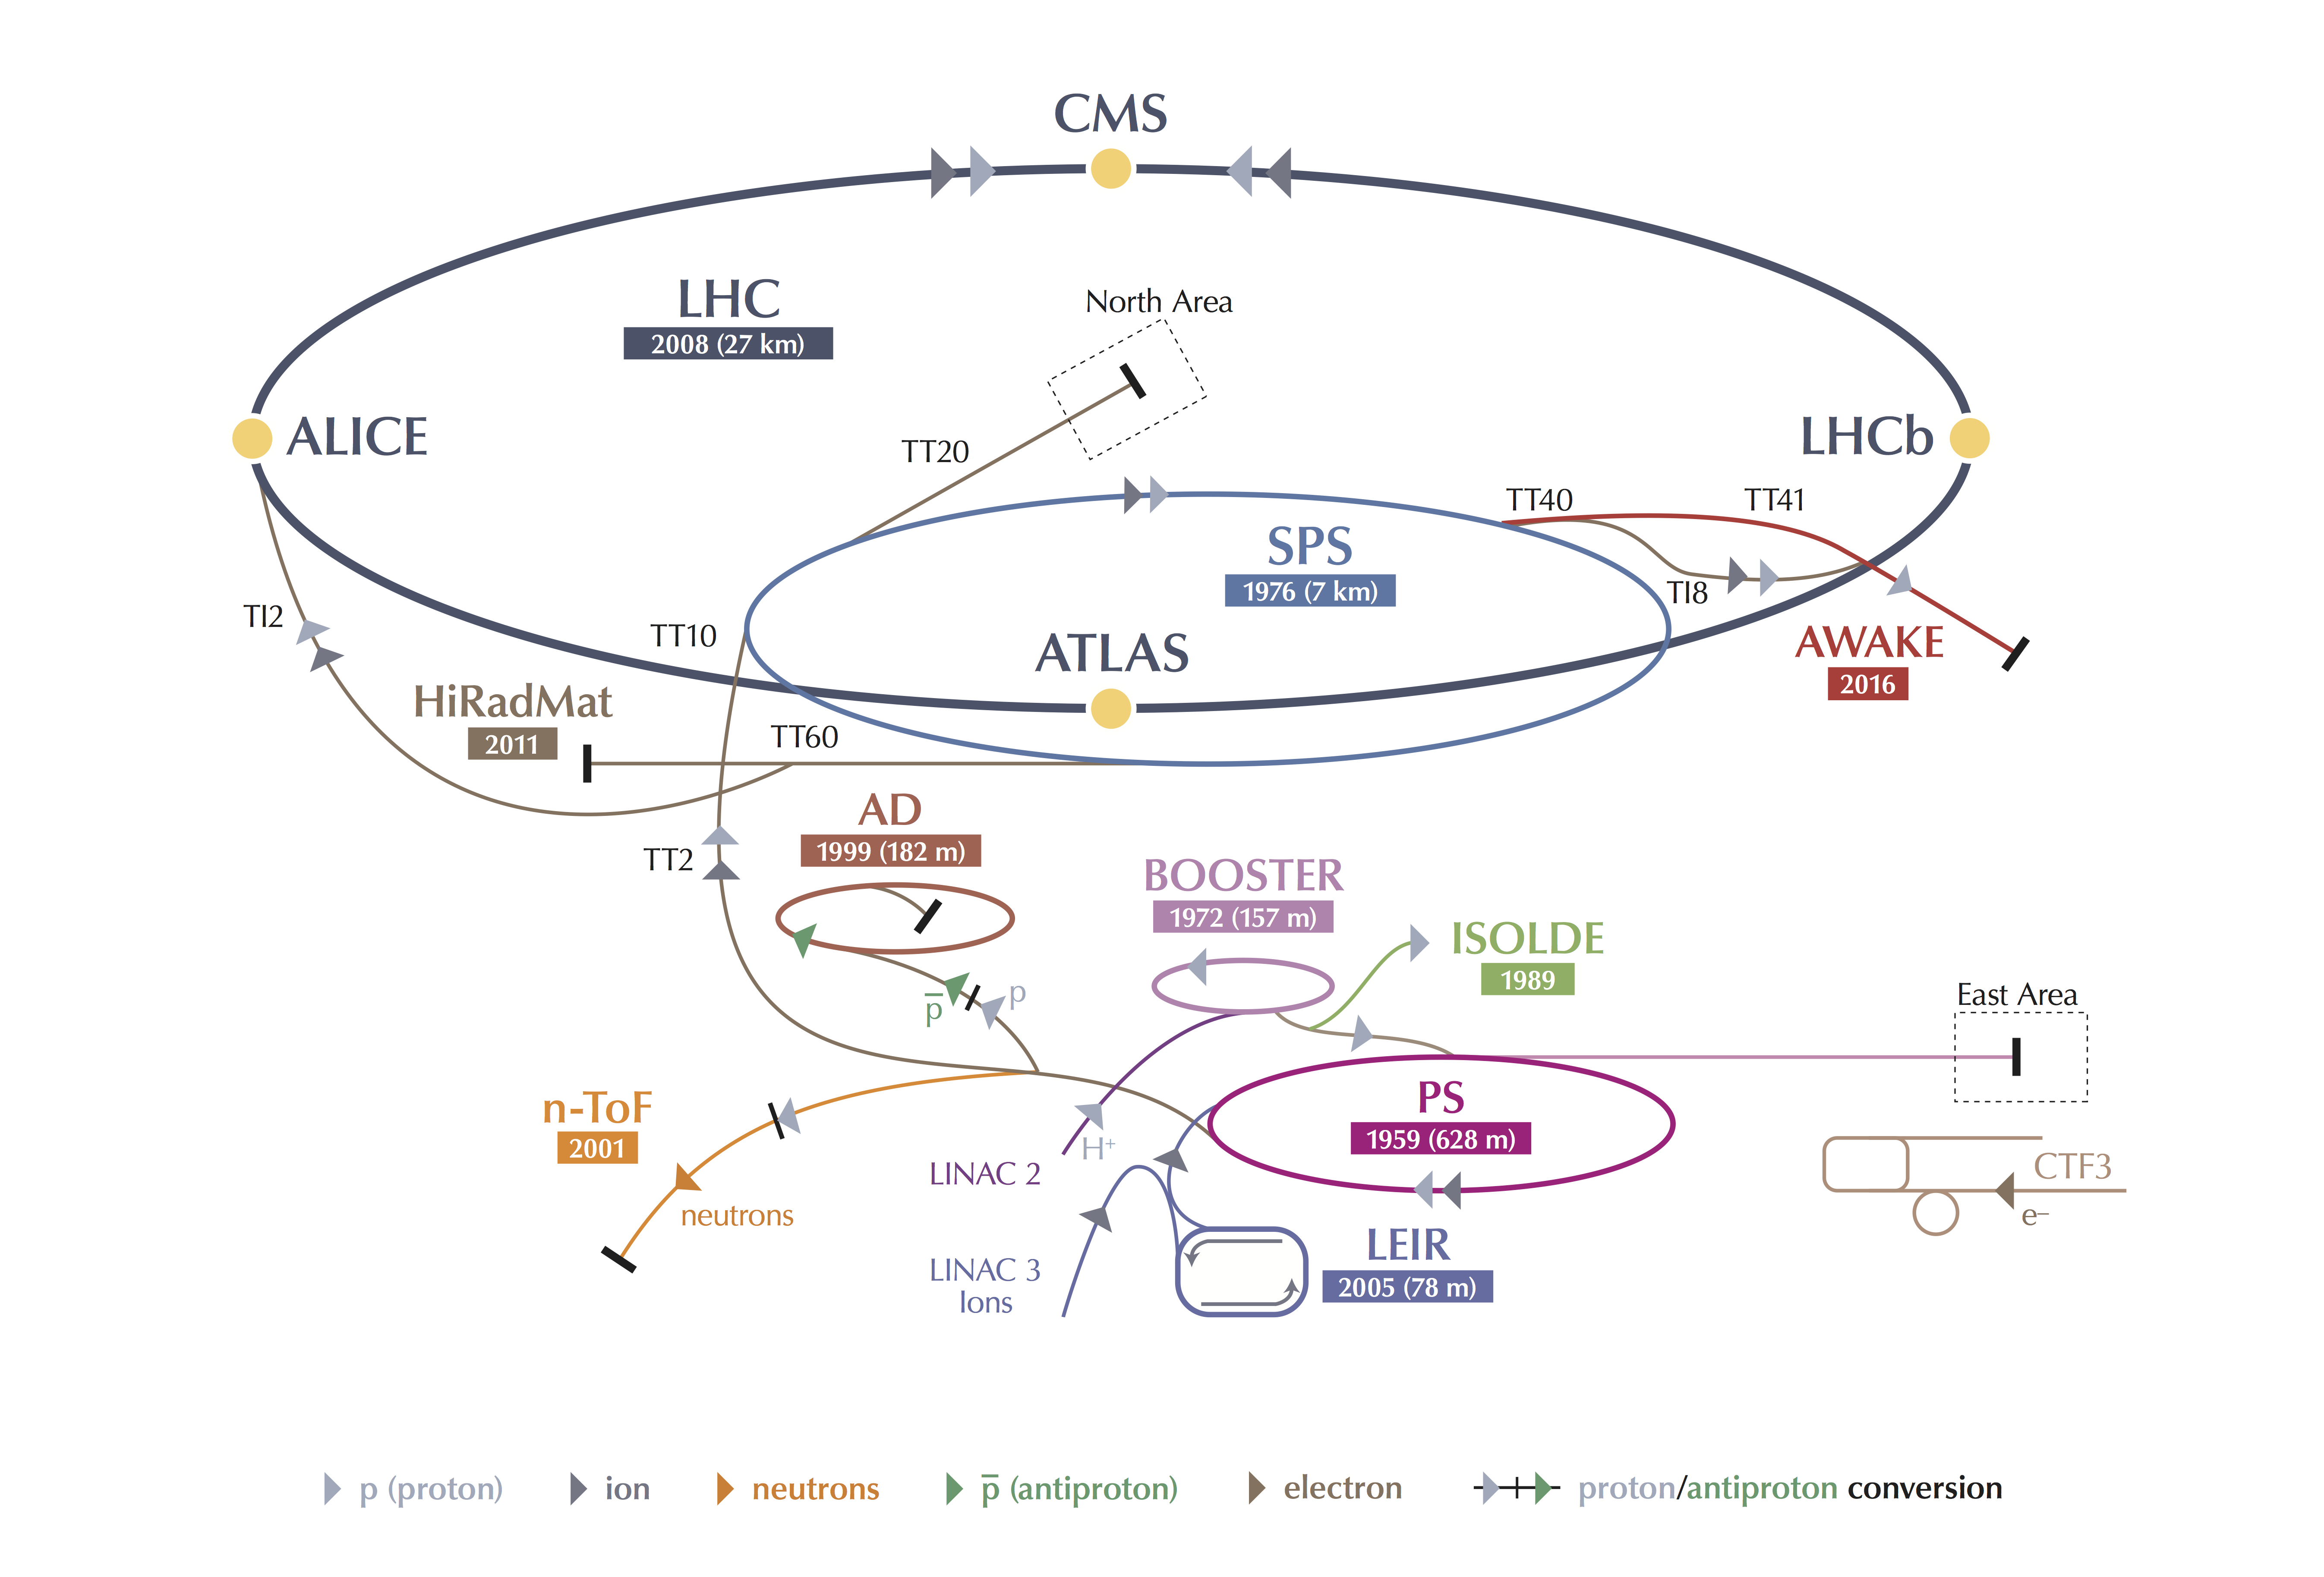
\includegraphics[width=1.0\columnwidth]{figures_chapter2/cern_complex.jpg}
\caption{A schematic representation of the CERN accelerator complex\cite{Haffner:1621894}.}
\label{fig:cern}
\end{figure}

Using the synchrotron method the design beam energy is achieved with $1232$ dipole magnets (15 meters in length) with a peak dipole field of $8.33$ Tesla. Quadrupole magnets (492) of $5-7$ meters in length are used to focus the beams. Two beam pipes with counter rotating beams are required as the LHC is a particle-particle accelerator.  Space limitations in the tunnels led to the adoption of the twin-bore\cite{Blewett:1971zzb} magnet design where the beam pipes are magnetically coupled and the magnets share the same mechanical structure and cryostat. The target magnetic field is achieved using niobium-titanium superconducting electromagnets with operating temperatures of $1.9$ K. Superfluid helium is used to cool the magnets to the operating temperature.   

\begin{figure}[h]
\centering
%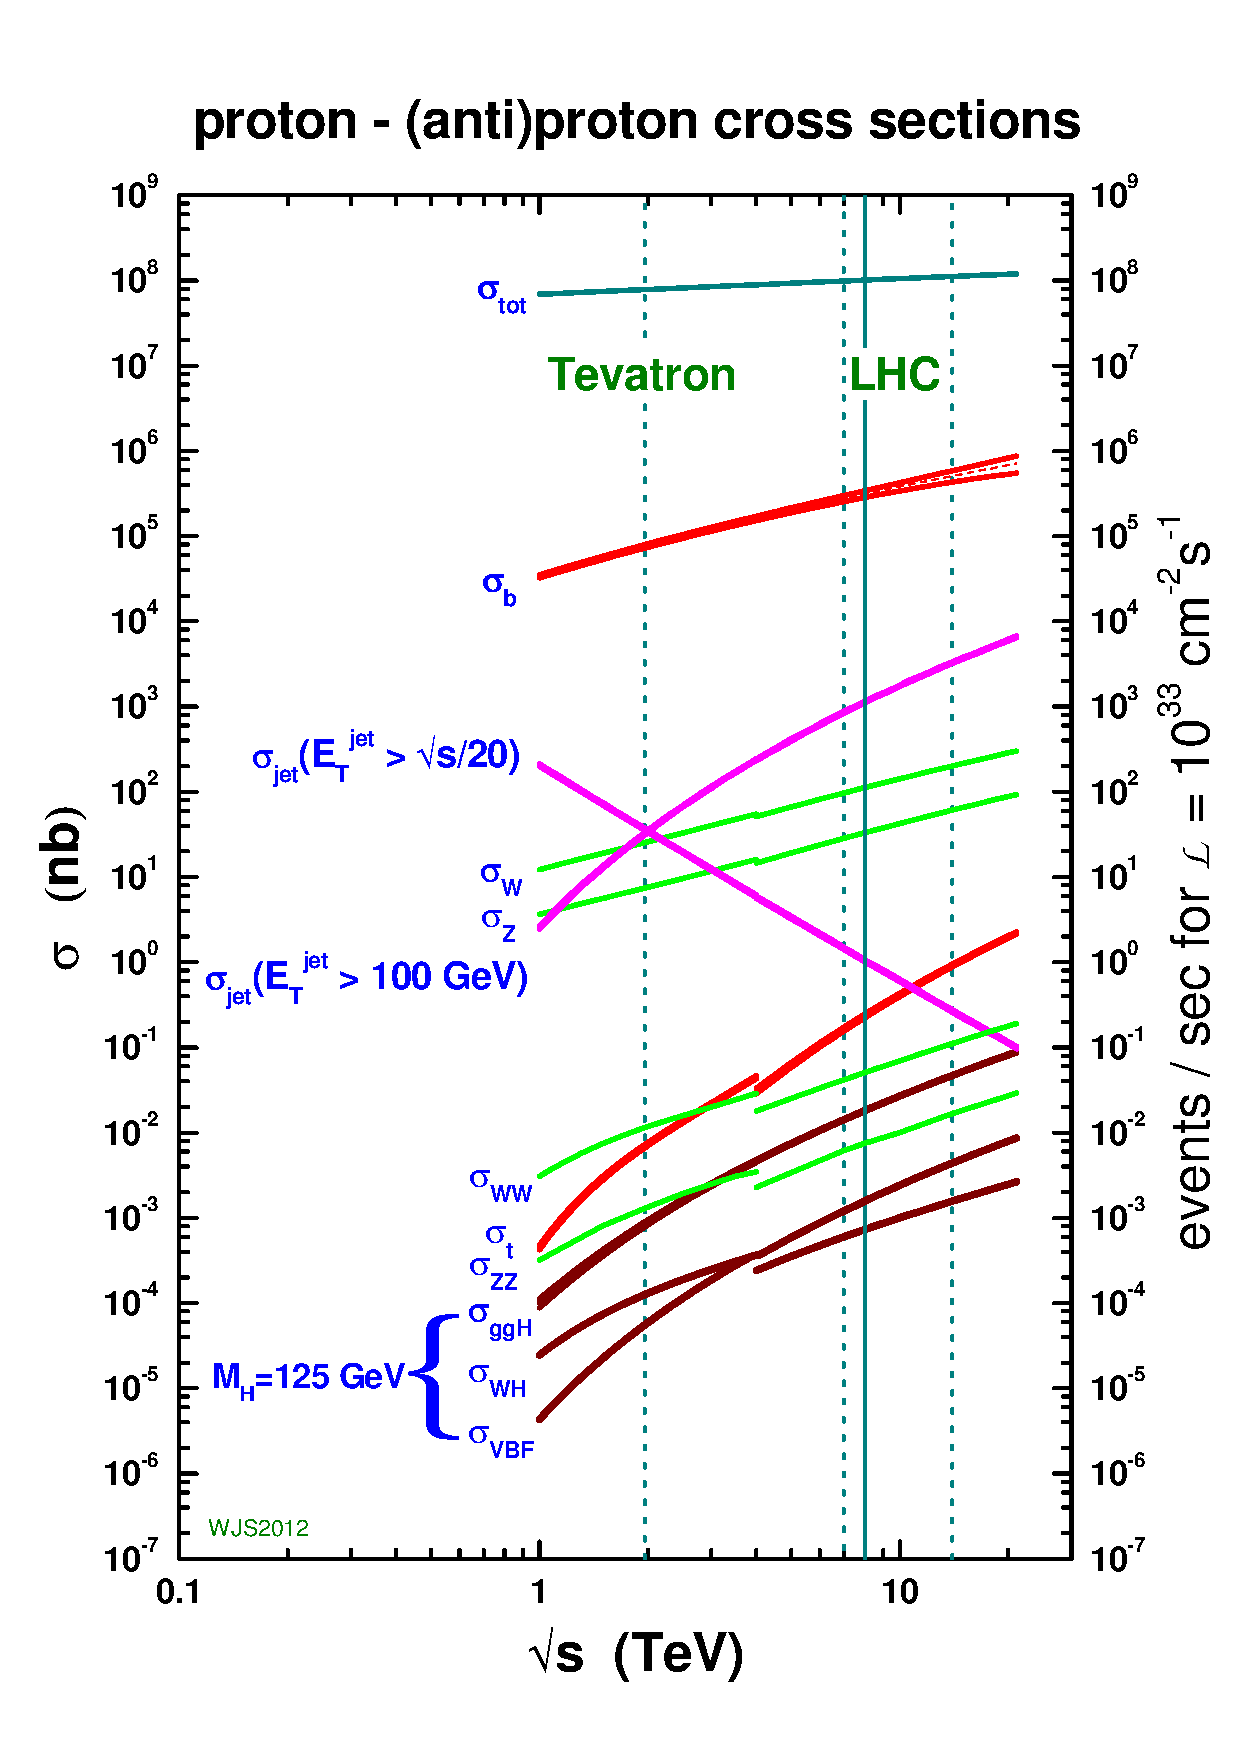
\includegraphics[width=1.0\columnwidth]{figures_chapter2/crosssections2013}
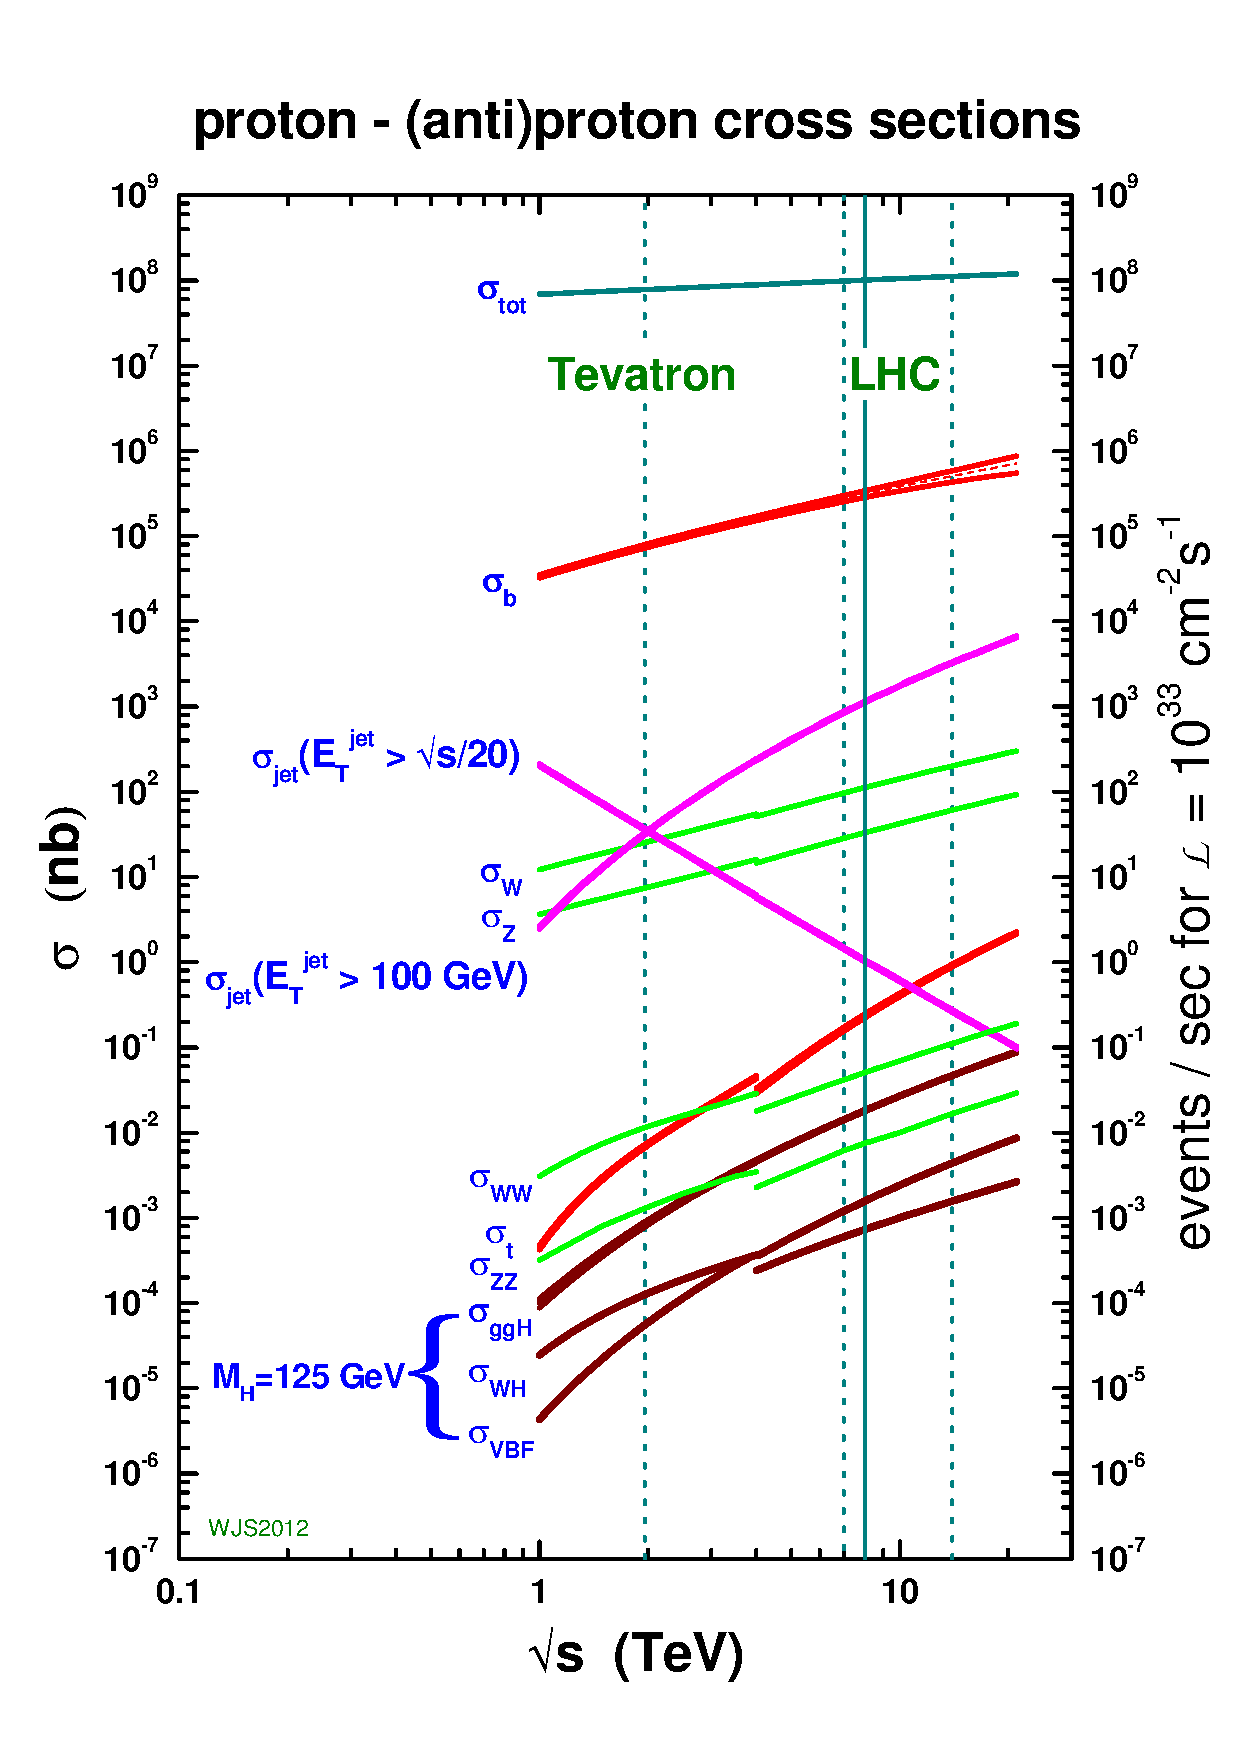
\includegraphics[width=0.6\textwidth]{figures_chapter2/crosssections2013}
\caption{Cross sections of various SM processes as a function of $\sqrt{s}$ in proton-proton and proton-antiproton collisions\cite{sterling}. The total hadronic cross section is based on a parameterization from Particle Data Group\cite{Agashe:2014kda}. The remaining cross sections are calculated at NLO or NNLO using MSTW2008 parton distributions\cite{MSTW}. The discontinuities illustrate the differences in cross sections between the proton-proton and proton-antiproton collisions.}
\label{fig:xsec}
\end{figure}

The goal of the LHC is to elucidate the mechanism of the EWSB and to look for hints of the BSM physics. The rate of events generated in the LHC collisions is given by 
\begin{equation} \label{eq:lumi}
N = \sigma L,
\end{equation}
where $\sigma$ is the cross section of the event under study and $L$ is the luminosity. Figure~\ref{fig:xsec} shows the production cross sections of various SM processes as a function of $\sqrt{s}$ in proton-proton and proton-antiproton collisions. The rear processes of interest at the LHC are orders of magnitude smaller than the total hadronic cross section. Therefore, in addition to high beam energies, high beam intensities are required. The design peak luminosity at the LHC is $10^{34}$ cm$^2$s$^{-1}$ for the proton-proton collisions. The high beam intensity requirement excludes the feasibility of using proton-antiproton collisions at the LHC. 


\begin{figure}[h]
\centering
%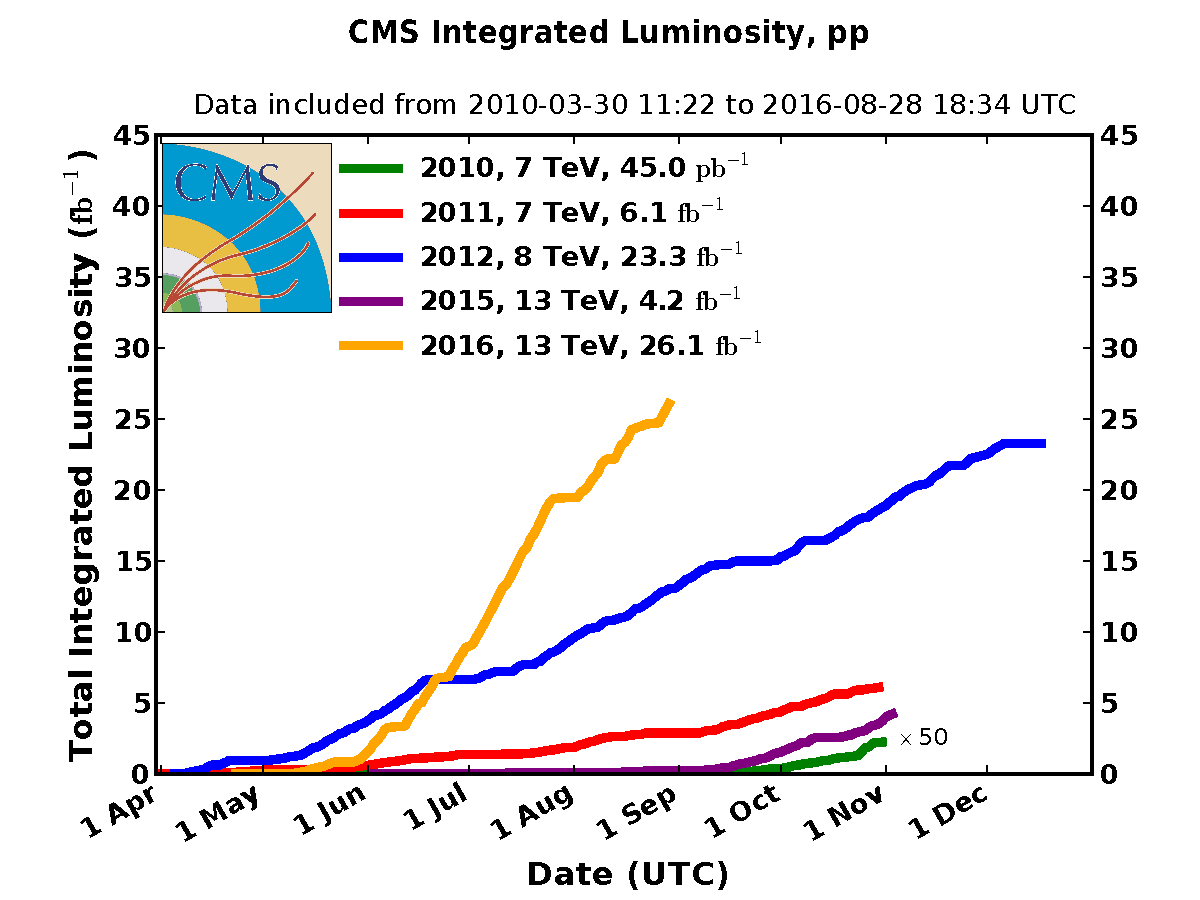
\includegraphics[width=1.0\columnwidth]{figures_chapter2/int_lumi_cumulative_pp_2}
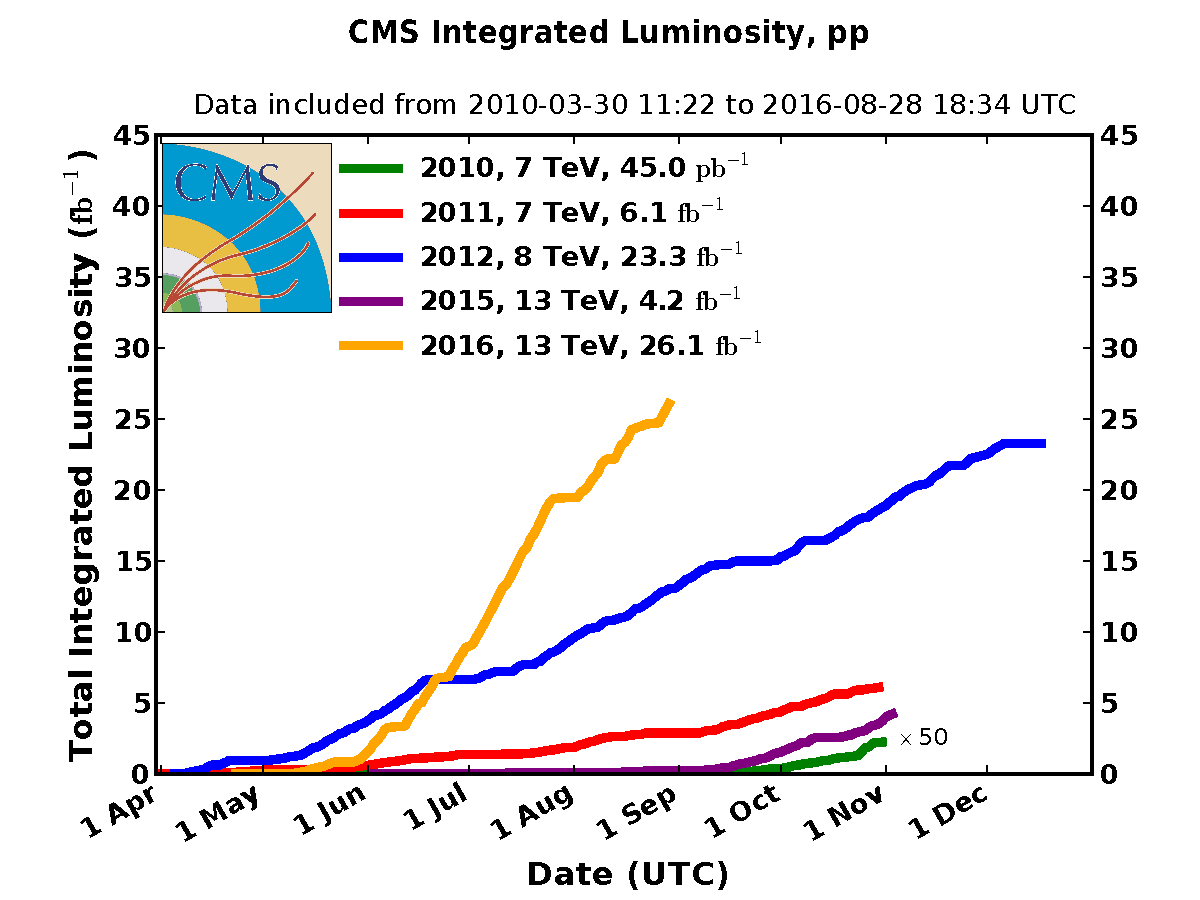
\includegraphics[width=0.8\textwidth]{figures_chapter2/int_lumi_cumulative_pp_2}
\caption{The total integrated luminosity delivered to CMS during stable beams in proton-proton collisions\cite{lumi_plot}. It is shown for $2010$ (green), $2011$ (red), $2012$ (blue), $2015$ (purple), and $2016$ (orange) data taking periods. The total integrated luminosity is shown for the data collected up to the end of August for the 2016 data taking period.} 
\label{fig:int}
\end{figure}

The machine luminosity depends only on the beam parameters. For a Gaussian beam distribution the dependance is given by
\begin{equation} \label{eq:lumi_beam}
L = \frac{N_{b}^2n_bf_{rev}\gamma_{r}}{4\pi\epsilon_n\beta^{*}}F,
\end{equation}
where $N_b$ is the number of particle per bunch ($\mathcal{O}(10^{11})$), $n_b$ is the number of bunches per beam, $f_{rev}$ is the revolution frequency, $\gamma_r$ is the relativistic gamma factor, $\epsilon_n$ is the normalized transverse beam emittance, $\beta^{*}$ is the beta function at the collision point, and $F$ is the geometric luminosity reduction factor due to the crossing angle at the interaction point.  The LHC has four interaction points that host ALICE\cite{Aamodt:2008zz}, ATLAS\cite{Aad:2008zzm}, CMS\cite{Chatrchyan:2008aa}, and LHCb\cite{Alves:2008zz} detectors. The ATLAS and CMS are general purpose, high luminosity experiments. The LHCb is a forward detector specializing in heavy flavor physics. The ALICE experiment is designed to study heavy-ion collisions.   


Figure~\ref{fig:int} shows the total integrated luminosity delivered to CMS during stable beams from October, $2010$ to August, $2016$ data taking periods. The LHC delivered proton-proton collisions at $\sqrt{s}$ of $7~\TeV$ during $2010$ and $2011$. The total integrated luminosity delivered in $2011$ was $6.1~\ifb$ with a peak instantaneous luminosity of $4.0 \times 10^{33}$ cm$^2$ s$^{-1}$. The luminosity recorded and certified, where all the detector sub-components are confirmed to operate normally, for physics results was $5.1~\ifb$. $\sqrt{s}$ was increased to $8~\TeV$ in $2012$ with $23.3~\ifb$ total integrated luminosity delivered to CMS with a peak instantaneous luminosity of $7.7 \times 10^{33}$ cm$^2$ s$^{-1}$. The total certified data amounted to $19.7~\ifb$. A bunch spacing of $50$ ns was used in the $2011$ and $2012$ data taking periods. 

 \begin{figure}[h]
\centering
%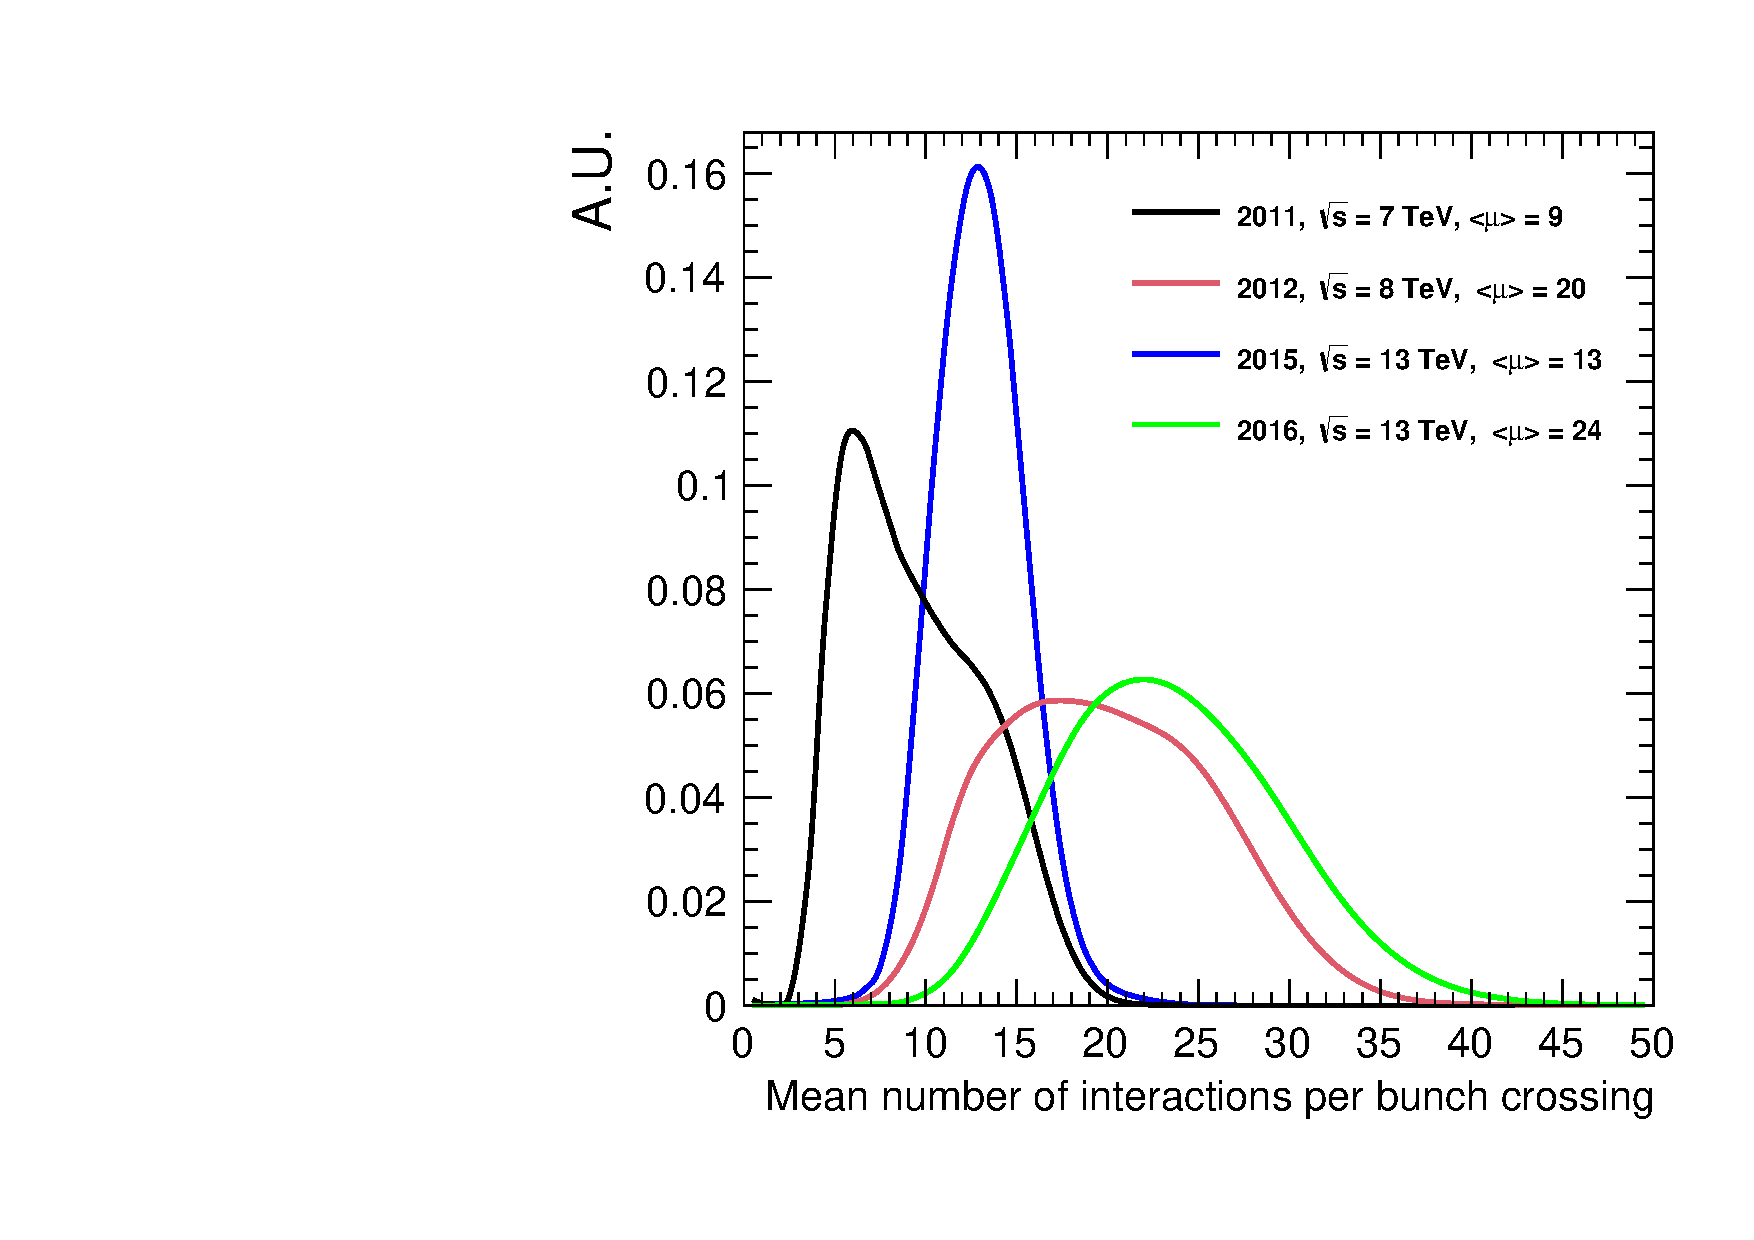
\includegraphics[width=1.0\columnwidth]{figures_chapter2/pileup_cms}
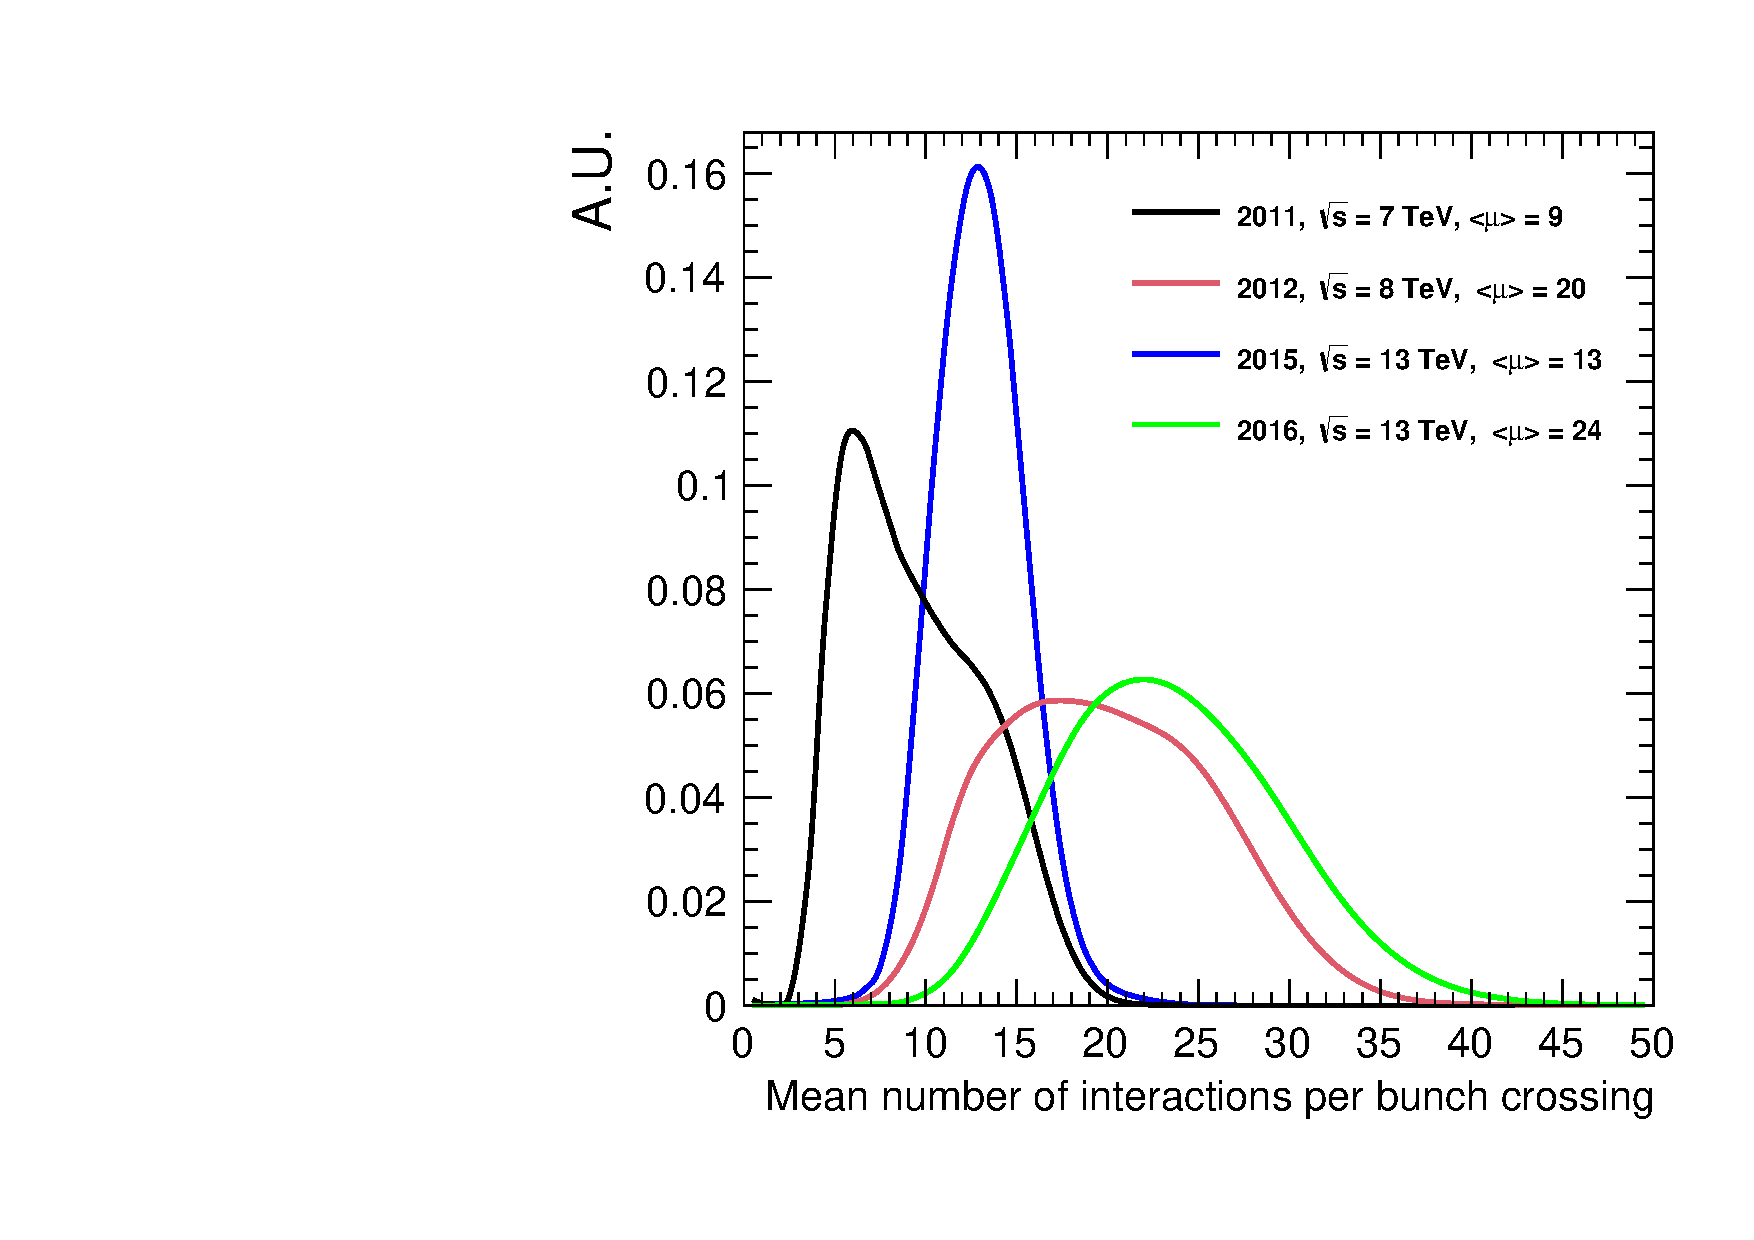
\includegraphics[width=0.6\textwidth]{figures_chapter2/pileup_cms}
\caption{Mean number of interactions per bunch crossing in proton-proton collisions. A detailed description of the  luminosity measurements in CMS can be found here\cite{CMS-PAS-LUM-13-001,CMS-PAS-LUM-15-001}. The distributions are shown for $2011$ (black), $2012$ (red), $2015$ (blue), and $2016$ (green) data taking periods.}
\label{fig:pu}
\end{figure} 

The LHC entered the Long Shutdown $1$ (LS1) in $2013$ for maintenance and upgrades during which the CMS detector was upgraded as well. The data taking resumed in $2015$ with $4.2~\ifb$ total integrated luminosity delivered to CMS with a peak instantaneous luminosity of $5.1 \times 10^{33}$ cm$^2$ s$^{-1}$. The LHC started to operate with the nominal bunch spacing of $25$ ns during this period. The total certified data for the nominal CMS operation and bunch spacing of $25$ ns amounted to $2.3~\ifb$. The data taking continued in $2016$ with an excellent performance by the LHC with significantly lower transverse beam sizes. This was achieved using a new bunch production scheme which resulted in a peak luminosity of  $1.2 \times 10^{34}$ cm$^2$ s$^{-1}$. Total integrated luminosity of $26.1~\ifb$ was delivered by the end of August of $2016$.   

Figure~\ref{fig:pu} shows the mean number of additional inelastic proton-proton interactions per bunch crossing (pileup). The additional pileup interactions in events present challenges in reconstruction and identification of the particles originating from the hard scattering of interest. The average number of pileup interactions in $2011$ was $9$ as the instantaneous luminosity continuously increased during the year. The average number of pileup interactions further increased to $20$ in $2012$ and reached to $24$ during $2016$.  While higher instantaneous luminosities are desired to enhance the production of the number events of interest, the effects of pileup need to be mitigated to improve the sensitivity of the results. 

%\subsection{Post Multiply Normalization}


